\documentclass[a4paper]{article}

%% Language and font encodings
\usepackage[english]{babel}
\usepackage[utf8x]{inputenc}
\usepackage[T1]{fontenc}
%% Sets page size and margins
\usepackage[a4paper,top=3cm,bottom=2cm,left=3cm,right=3cm,marginparwidth=1.75cm]{geometry}

%% Useful packages
\usepackage{amsmath}
\usepackage{graphicx}
\usepackage[colorinlistoftodos]{todonotes}
\usepackage[colorlinks=true, allcolors=black]{hyperref}
\usepackage{tabularx,ragged2e,booktabs,caption}

\usepackage{appendixnumberbeamer}

\usepackage{listings}
\usepackage{color}

\definecolor{dkgreen}{rgb}{0,0.6,0}
\definecolor{gray}{rgb}{0.5,0.5,0.5}
\definecolor{mauve}{rgb}{0.58,0,0.82}

\lstset{frame=tb,
  language=Java,
  aboveskip=3mm,
  belowskip=3mm,
  showstringspaces=false,
  columns=flexible,
  basicstyle={\small\ttfamily},
  numbers=none,
  numberstyle=\tiny\color{gray},
  keywordstyle=\color{blue},
  commentstyle=\color{dkgreen},
  stringstyle=\color{mauve},
  breaklines=true,
  breakatwhitespace=true,
  tabsize=3
}

\title{Implémentation du protocole DES au travers d'un
pipeline de tâches ADA\\ \small{Sous la direction d'Emmanuel CAGNIOT}}
\author{Vadim MIKA - Master 1 SSI \\Université de Caen Normandie}
\date{Avril 2018}

\begin{document}

\maketitle

\newpage

\tableofcontents

\newpage


\section{Introduction}

\subsection{Présentation générale du projet}
L'objectif de ce projet est d'implémenter l'algorithme DES (\emph{D}ata \emph{E}ncryption \emph{S}tandard), un algorithme de chiffrement de données utilisé jusqu'en 1999 puis remplacé en 2001 par AES. Dans un premier temps, l'algorithme sera implémenté dans une version séquentielle puis parallélisé dans une seconde version.
\smallbreak
Le langage de programmation utilisé pour implémenter cet algorithme est le langage Ada sous sa norme 2012

\subsection{Enjeux du projet}
L'enjeu de ce projet est double :
\begin{itemize}
\item Implémenter de manière séquentielle et parallèle l'algorithme de chiffrement de données DES
\item Apprendre le langage Ada sous sa norme 2012 et tirer au maximum partie de ses fonctionnalités pour l'implémentation de l'algorithme
\end{itemize}

\subsection{Étapes du projet}
Ce projet s'est déroulé en trois étapes majeures : 
\begin{itemize}
\item Apprentissage des rudiments du langage Ada
\item Implémentation de l'algorithme dans une version séquentielle
\item Implémentation de l'algorithme dans une version parallèle
\end{itemize}

\section{Présentation de l'algorithme DES}
Le DES est un algorithme de chiffrement à bloc. Il applique une série de filtres à chaque bloc de bits afin de le chiffrer puis de l'insérer dans le document de sortie.
\smallbreak
La clé permettant de chiffrer les données est composée de 56 bits. Elle est dérivée en 16 clés de 46 bits chacune permettant d'effectuer un des cycles de chiffrements. Le fonctionnement général de l'algorithme DES est donc le suivant :
\begin{itemize}
\item Transposition
\item Cycles de chiffrements (au nombre de 16)
\item Échange gauche-droite
\item Transposition inverse
\end{itemize}

\begin{figure}
\begin{center}
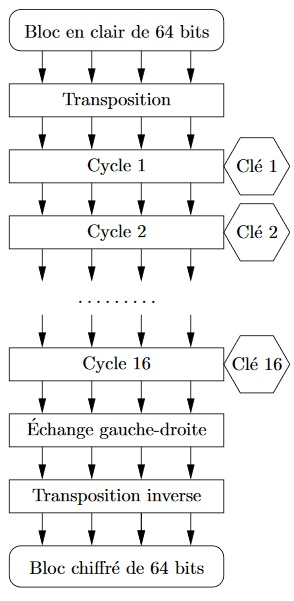
\includegraphics[scale=0.5]{images/des_structure.png} 
\caption{Schéma général de l'algorithme DES}
\end{center}
\end{figure}
\medbreak

Afin de comprendre le principe général de l'algorithme, on expliquera succinctement les étapes le composant.

\subsection{Transposition initiale}
Comme dans la plupart des algorithmes de chiffrement à bloc, on utilise des permutations de mantisses binaires afin de chiffrer les données. Les permutations (ou arrangements) ont l'avantage d'être déterministes et facilement inversibles. La transposition initiale de l'algorithme DES est définie par le tableau suivant : 


\begin{table}[h]
\centering
\begin{tabular}{|cccccccc|}
  \hline
  58 & 50 & 42 & 34 & 26 & 18 & 10 & 2 \\
  60 & 52 & 44 & 36 & 28 & 20 & 12 & 4 \\
  64 & 56 & 48 & 40 & 32 & 24 & 16 & 8 \\
  57 & 49 & 41 & 33 & 25 & 17 & 9 & 1 \\
  59 & 51 & 43 & 35 & 27 & 19 & 11 & 3 \\
  61 & 53 & 45 & 37 & 29 & 21 & 13 & 5 \\
  63 & 55 & 47 & 39 & 31 & 23 & 15 & 7 \\
  \hline
\end{tabular}
\caption{Tableau des indices de la permutation initiale de DES}
\end{table}
\smallbreak
Ce tableau définit la permutation des bits du bloc d'entrée. La première case contient la valeur 58 ce qui signifie que le bit de position 1 du bloc permuté sera le bit de position 58 du bloc de départ. Une fois les 64 permutations effectués, on envoie le bloc suivant dans le prochain filtre.

\subsection{Cycles de chiffrements}
L'algorithme DES est composé de 16 cycles de chiffrements, réalisés à l'aide d'un réseau de Feistel. Un réseau de Feistel (nommé d'après le cryptologue d'IBM Horst Feistel) est un construction utilisée dans les algorithmes de chiffrement à bloc. Elle offre certains avantages dont la ressemblance (voire similitude) de l'architecture de chiffrement et de déchiffrement ou encore une certaine robustesse à la cryptanalyse linéaire grâce à l'utilisation d'une fonction cryptographique.

\smallbreak
\begin{figure}
\begin{center}
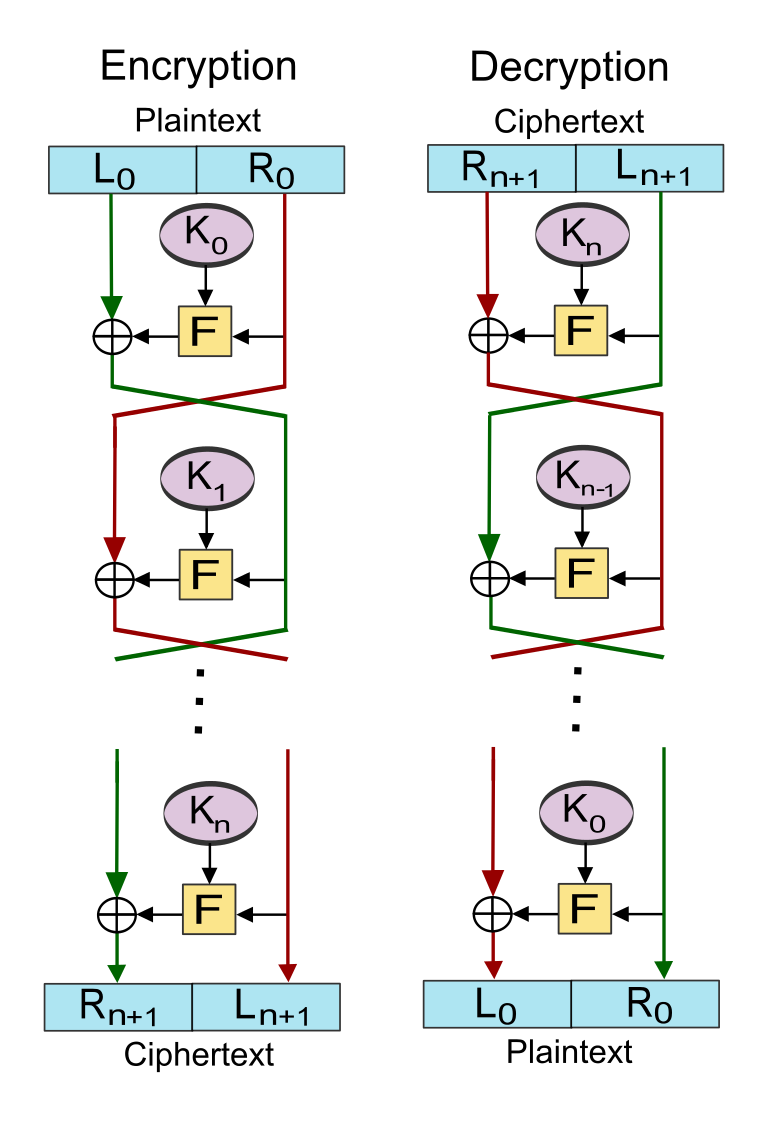
\includegraphics[scale=0.2]{images/feistel_network.png} 
\caption{Schéma général de l'algorithme DES}
\end{center}
\end{figure}

\smallbreak
Un cycle est décomposé en 4 étapes :
\begin{itemize}
\item Séparation du bloc d'entrée en demi-bloc de longueurs égales
\item Mixage non-linéaire avec la sous-clé correspondante au cycle via la fonction cryptographique
\item Mixage linéaire avec le second demi-bloc
\item Permutation des blocs
\end{itemize}
\smallbreak
\newpage

En général, les fonctions cryptographiques se veulent non-linéaire afin d'éviter les études cryptographiques linéaires. En effet si en modifiant un seul bit en entrée et que la sortie reste quasiment identique, on peut déduire des informations sur le message de départ. En l'occurrence on pourrait déduire que les deux messages à chiffrer sont quasiment identiques. Les fonctions cryptographiques recherchent donc à accomplir ce qu'on appelle un effet avalanche élevé. Un effet avalanche est la propriété d'une fonction à produire des résultats complètement différents pour des entrées quasiment identiques.
\smallbreak
Dans le cas de la fonction cryptographique de DES, l'effet avalanche est produit par différentes permutations et surtout un réseau de permutation via des entités appelés S-Boxes.

\subsubsection{Fonction cryptographique de DES}
La fonction cryptographique de DES est divisée en 3 étapes :
\begin{itemize}
\item Expansion du demi-bloc d'entré et mixage linéaire avec la sous-clé du cycle
\item Substitutions du bloc via S-Boxes
\item Permutation finale 
\end{itemize}

\paragraph{Expansion}
\smallbreak
La première étape de la fonction cryptographique de DES est l'expansion du demi bloc. En effet afin de pouvoir mixer le bloc avec la clé, il est nécessaire d'avoir des unités binaires de même taille. Or le demi-bloc est composé de 32 bits et la sous-clé est composé de 48 bits. Ainsi, il est nécessaire d'augmenter la taille du demi-bloc d'entrée. Pour cela, on procède de manière analogue à la permutation de départ. Ci-dessous la table d'expansion du bloc de départ :

\begin{table}[h]
\centering
\begin{tabular}{|cccccc|}
  \hline
  32 & 1 & 2 & 3 & 4 & 5 \\
  4 & 5 & 6 & 7 & 8 & 9 \\
  8 & 9 & 10 & 11 & 12 & 13 \\
  12 & 13 & 14 & 15 & 16 & 17 \\
  16 & 17 & 18 & 19 & 20 & 21 \\
  20 & 21 & 22 & 23 & 24 & 25 \\
  24 & 25 & 26 & 27 & 28 & 29 \\
  28 & 29 & 30 & 31 & 32 & 1 \\
  \hline
\end{tabular}
\caption{Tableau de l'expansion du bloc de départ de la fonction cryptographique de DES}
\end{table}

\smallbreak
\newpage

\paragraph{Substitution}
La deuxième étape de la fonction cryptographique de DES est la substitution des bits du bloc. Cette substitution est effectuée à l'aide de S-Boxes. Les S-Boxes sont des tableaux permettant la substitution des bits et la réduction d'une entrée de 48 bits à une entrée de 32 bits.
\smallbreak
Une S-Box est un tableau qui selon les 6 bits d'entrée ressort 4 bits. Afin de connaître les bits de sortie, il suffit de regarder les 2 bits extérieurs et se placer sur la ligne correspondante. Ensuite on regarde les 4 bits centraux et on en déduit la colonne correspondante. En croisant la ligne et la colonne obtenue, on obtient les 4 bits de sortie. En tout, il y a 8 S-Boxes, une pour chaque mot de 8 bits de l'entrée.

\begin{figure}[h]
\begin{center}
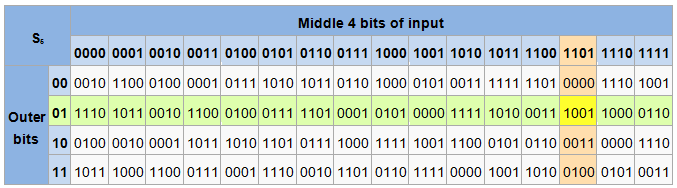
\includegraphics[width=\textwidth]{images/SBox6.png} 
\caption{Exemple de la SBox 6}
\end{center}
\end{figure}

\paragraph{Permutation}
La dernière étape de la fonction cryptographique de DES est la permutation. Encore une fois, cette permutation est définie par un tableau. Ci-dessous le tableau de la permutation finale :
\begin{table}[h]
\centering
\begin{tabular}{|cccc|}
  \hline
  16 & 7 & 20 & 21 \\
  29 & 12 & 28 & 17 \\
  1 & 15 & 23 & 26 \\
  5 & 18 & 31 & 10 \\
  2 & 8 & 24 & 14 \\
  32 & 27 & 3 & 9 \\
  19 & 13 & 30 & 6 \\
  22 & 11 & 4 & 25 \\
  \hline
\end{tabular}
\caption{Tableau de la permutation de la fonction cryptographique de DES}
\end{table}

\subsection{Génération de sous-clés}
Comme vu précédemment, les cycles de chiffrements nécessitent chacun une clé afin de l'utiliser dans la fonction de chiffrement. Afin de dériver 16 sous-clés de la clé initiale, on procède de la manière suivante :
\begin{itemize}
\item Récupération de la clé initiale (56 bits + 8 bits de parités)
\item Permutation $PC1$ des 56 bits
\item Séparation de la clé en demi-bloc de 28 bits
\item Left-shift de chaque demi-bloc en fonction du round
\item Reconstruction et permutation $PC2$ du bloc final
\end{itemize}

Ainsi, on peut obtenir 16 clés de 48 bits à partir d'une clé de 56 bits. On peut observer que la sous-clé $k+1$ est déterminée grâce au bloc $k$ qui a subi un left shift. Les left shift correspondent à l'opération élémentaire de décalage à gauche d'un registre. De plus, le nombre de left-shift change en fonction de l'indice de la sous-clé générée. Pour les rounds 1, 2, 9 et 16 on effectue une seul left-shift. Pour tous les autres on en effectue 2.
\smallbreak
Ci-dessous le schéma général de génération de sous-clés :
\begin{figure}[h]
\begin{center}
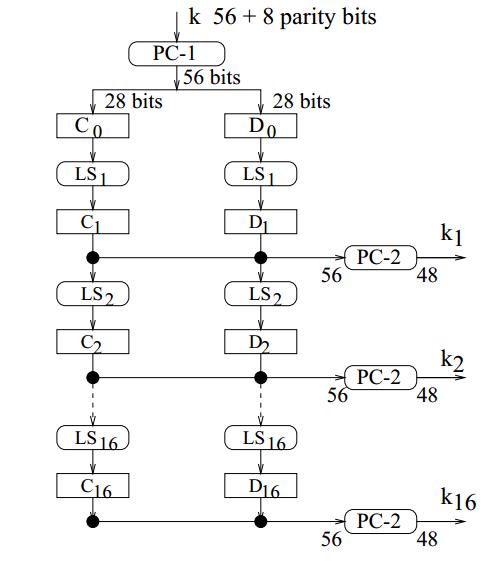
\includegraphics[scale=0.5]{images/key.png} 
\caption{Schéma du circuit de génération de sous-clés}
\end{center}
\end{figure}

\subsection{Phase finale de l'algorithme et circuit de chiffrement/déchiffrement}
La dernière étape de l'algorithme DES est l'échange gauche droite des derniers blocs et la transposition finale. L'échange gauche-droite est la simple permutation des demi-bloc finaux à la fin des 16 cycles de chiffrements. La transposition inverse est l'inverse des index de la transposition initiale.
\smallbreak
A la fin de ce circuit, on obtient un bloc chiffré ou déchiffré. Pour obtenir un texte ou contenu binaire complètement chiffré il suffit d'exécuter ce traitement sur chaque bloc. Le déchiffrement d'un texte  est assez simple grâce au réseau de Feistel qui permet de simplement de changer l'ordre de clés (sous-clé 16 pour le premier cycle, sous-clé 15 pour le second) afin d'obtenir un texte déchiffré.
\smallbreak
Voyons maintenant comment implémenter cet algorithme de manière séquentielle dans le langage de programmation Ada.


\section{Présentation du langage Ada}

\subsection{Philosophie et origine du langage}
Le langage Ada est un langage de programmation orienté objet dont les premières versions remontent au début des années 1980 conçu par l'équipe \emph{CII-Honeywell Bull} dirigé par Jean Ichbiah en réponse à un cahier des charges établi par le département de la Défense des États-Unis. Ce langage suit une philosophie assez différente de celle d'autres langages de programmation.
\smallbreak
Le langage Ada a été conçu pour être le plus robuste possible. Parmi ses fonctionnalités on retrouve des fonctionnalités classiques de beaucoup de langages de programmations comme la généricité, le typage statique ou encore la notion de module et de paquetages. Cependant certaines fonctionnalités du langage permettent de restreindre les capacités l'utilisateur afin d'avoir un comportement aussi déterministe que possible.
\smallbreak

Il est également possible de déclarer des types et d'accéder à des fonctionnalités bas-niveau permettant de décrire des paramètres fin de représentations des entités en mémoire. Il est notamment possible de définir la taille en mémoire d'un type afin d'être certain de sa représentation concrète.
\smallbreak
Plus généralement, le langage est conçu pour avoir une robustesse à toute épreuve et avoir un le comportement le plus déterministe possible.

\subsection{Portée du langage}
Même si ce langage permet de réaliser des projets orientés objets classiques, il a été conçu avec certaines fonctionnalités comme la notion de multi-tâche, programmation en temps réel ou encore la programmation par contrat qui lui donne la caractéristique d'être un langage fiable et robuste. Certaines fonctionnalités comme le profil \emph{Ravenscar} permettent d'établir des preuves formelles de fonctionnement du programme.
\smallbreak
En conclusion, même si le langage Ada contient toutes les fonctionnalités des langages classiques, il se destine aux programmes nécessitant une haute fiabilité d'exécution ou souhaitant tirer partie des fonctionnalités permettant la programmation parallèle.

\section{Première implémentation : modélisation objet}

Une fois l'algorithme défini, on peut étudier sa structure de manière plus approfondie. L'algorithme est une succession de traitements sur des blocs de 64 bits. Plus concrètement, on pourrait définir un objet ayant pour charge un seul traitement pour un bloc en question. Ainsi, on pourrait définir une chaîne de travail ou chaque objet traite le bloc et passe le bloc traité au filtre suivant. 

\subsection{Architecture générale du programme}
Pour mettre en place cet algorithme de manière séquentielle, on a recours au design pattern \emph{Chain of Responsibility}. Ce pattern décrit un comportement permettant de définir une suite de tâche à effectuer.

\begin{figure}[h]
\begin{center}
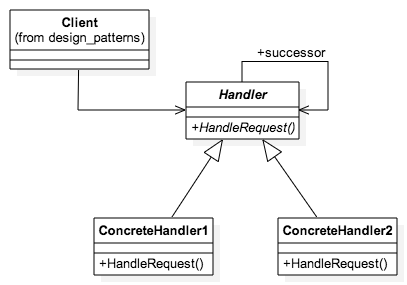
\includegraphics[scale=0.5]{images/CoR.png} 
\caption{Design pattern Chain of Responsibility}
\end{center}
\end{figure}

Ce design pattern permet de s'assurer de l'ordre d'exécution et de l'enchaînement des filtres à appliquer au bloc ainsi que de bien séparer les filtres en les encapsulant dans des objets.
\newpage


\subsection{Notion d'objet en Ada}
En Ada, contrairement à d'autres langages, la classe n'est pas la structure de base. En effet Ada utilise la notion de package afin de définir des objets. Un package peut contenir des types ou sous-types qui sont souvent des redéfinitions de type déjà existant (un bit est peut par exemple être représenté par un type Entier pouvant avoir comme valeur 0 ou 1). On peut associer un \texttt{Record} à un type Ada qui permet de lui assigner des attributs permanents pour le type ce qui permet de lui donner la composante d'Objet.
\smallbreak
Finalement, on pourrait définir un objet Ada comme un type possèdant un \texttt{Record} et possédant au moins une primitive. Il peut donc être décomposé en 3 parties : 
\begin{itemize}
\item Un type qui définit le typage de l'objet (\texttt{array},\texttt{integer} ou un type arbitraire défini par l'utilisateur)
\item Un \texttt{record} (optionnel)
\item Des méthodes associées au packages ou au type lui même
\end{itemize}
\smallbreak
Les droits d'accès peuvent être gérés en Ada de la même manière que dans d'autres langages, on peut définir des méthodes ou attributs privés pour un objets et ainsi gérer les interactions possibles inter-objets ou utilisateurs-objets. Ci-dessous l'exemple d'un type classique Ada.

\begin{lstlisting}[language=Ada]
PACKAGE P_Pile IS
         --   PARTIE PUBLIQUE
   PROCEDURE Push (P : IN OUT T_Pile; N : IN Integer) ;
   PROCEDURE Pop (P : IN OUT T_Pile ; N : OUT Integer) ;
   FUNCTION Empty (P : IN T_Pile) RETURN Boolean ;
   FUNCTION Length(P : T_Pile) RETURN Integer ;   
   FUNCTION First(P : T_Pile) RETURN Integer ;

PRIVATE
         --   PARTE PRIVEE : NOS TYPES
   TYPE T_Cellule;
   TYPE T_Pile IS ACCESS ALL T_Cellule;
   TYPE T_Cellule IS

      RECORD
         Valeur  : Integer;
         Index   : Integer;
         Suivant : T_Pile; 
      END RECORD;
END P_Pile;
\end{lstlisting}

\subsection{Principe général de l'implémentation}
L'algorithme se déroule en 3 grandes étapes : 
\begin{itemize}
\item Lecture du fichier d'entrée et définition du conteneur de données binaires
\item Application des filtres
\item Écriture des données dans le fichier binaire de sortie
\end{itemize}

Une fois l'architecture générale définie, on peut mettre en place les objets caractérisant les filtres. Pour tirer partie des fonctionnalités du langage Ada, on va définir un objet définissant le comportement général d'un filtre et ses objets dérivés définissant le comportements de chaque filtres.


\subsection{Objet \texttt{Step\_Handler} général}
Comme on l'a vu auparavant, on aura recours au design pattern \texttt{Chain of Responsibility}. Il est donc nécessaire d'établir notre modèle de filtre. C'est le rôle du package \texttt{P\_StepHandler}. Ce filtre sera abstrait et n'aura comme rôle que de définir les attributs et les procédures/fonctions nécessaires et communs à tous les filtres concrets. La définition du "Handler" général est la suivante :
\smallbreak
\begin{lstlisting}[language=ada]

package P_StepHandler is
   
   type T_StepHandler   is abstract tagged private;
   type Ptr_Handler is access all T_StepHandler'Class;
      
   procedure Handle (Self : in out T_StepHandler) is abstract;
   procedure Set_NextHandler (Self            : in out T_StepHandler;
                              Ptr_StepHandler : Ptr_Handler);
   function Get_BinaryContainer (Self : in out T_StepHandler) 
                            return BinaryContainer_Access;
   procedure Set_BinaryContainer (Self : in out T_StepHandler;
                   Ptr_BinaryContainer : BinaryContainer_Access);

PRIVATE

   type T_StepHandler is abstract tagged
      record
         NextHandler      : access all T_StepHandler'Class;
         Ptr_BinaryContainer : BinaryContainer_Access;
      end record;

end P_StepHandler
\end{lstlisting}

Le types \texttt{StepHandler} et son pointeur associé sont les types nécessaires à la définition de notre objet. La procédure Handle est vouée à être redéfinie par tout les Handler concrets.
\smallbreak
Dans son \texttt{Record} on peut trouver les deux attributs que tous les Handler auront besoin pour fonctionner : 
\begin{itemize}
\item NextHandler : le prochain filtre dans la chaîne de responsabilité
\item Ptr\_BinaryContainer : le tableau de donnée binaire. Étant donné que Ada ne permet pas d'avoir des tableaux à longueur inconnue à la compilation (on n'a pas encore parcouru le fichier donc on ne connaît pas la longueur du tableau), on a recours à ce pointeur pour résoudre le problème.
\end{itemize}
Une fois ce type déclaré abstrait défini, on peut définir les Handler concrets qui permettront d'effectuer les traitements sur les blocs.


\subsubsection{\texttt{Input Handler}}
Ce maillon de la chaîne a pour rôle de scanner le texte d'entrée. Il parcourt la fichier caractère par caractère puis récupère son code Uniode (opération élémentaire Ada \texttt{Character'Pos}) et convertit cette valeur en binaire avant de l'ajouter au conteneur binaire principal. Son \texttt{NextHandler} est le \texttt{IPHandler}.

\subsubsection{\texttt{IP Handler}}
Ce maillon de la chaîne effectue le premier traitement de l'algorithme , la transposition initiale. Pour cela, le \texttt{Handler} parcourt tous le conteneur binaire principal et effectue la transposition. Pour cela, la \texttt{Handler} dispose du tableau d'indice correspondant à la transposition initiale décrite dans l'algorithme.

\subsubsection{\texttt{KeyGen Handler}}
Ce maillon a pour rôle de générer les clés nécessaires aux cycles de chiffrement. Il implémente l'algorithme de génération des clés décrit dans le standard DES. Une fois ces clés générées, il le met à disposition dans un \texttt{array} de clés et le rend disponible au \texttt{Handler} suivant : le \texttt{Feistel Handler}.

\subsubsection{\texttt{Feistel Handler}}
Ce maillon est de loin le plus long en terme de temps de traitement. Il exécute 16 cycles de chiffrements sur tous les blocs du conteneur binaire général. Il possède comme attribut un pointeur vers le conteneur de clés afin de chiffre les données du conteneur. Il exécute aussi l'échange gauche-droite final. Une fois son traitement achevé, il passe la main au  \texttt{Reverse IP Handler}

\subsubsection{\texttt{Reverse IP Handler}}
Ce maillon se base exactement sur le même principe que la transposition initiale. Ce \texttt{Handler} possède également un tableau d'indice nécessaire à la transposition. Une fois son traitement terminé, il passe la main au dernier maillon de la chaîne, le \texttt{OutputHandler}.

\subsubsection{\texttt{Output Handler}}
Ce maillon a pour but de décoder et insérer les informations binaires dans le fichier. Pour cela, il parcourt les blocs du conteneur binaire et décode leur valeur, puis les convertit en caractère et enfin les insère dans le fichier texte cible.

\subsection{Encapsulation de la chaîne de responsabilité}
Afin de traiter les demandes de l'utilisateur, on définit une classe \texttt{Des Handler} qui permet de gérer les opérations extérieures non gérées par les maillons de la chaîne.
\smallbreak
Le principal intérêt d'encapsuler la chaîne dans une classe est de permettre de gérer les paramètres de la chaîne comme par exemple l'ordre de lequel s'exécute les maillons. Il permet également de contourner les problématiques du langage Ada. En effet cette classe mère permet de parser le fichier de départ afin de déterminer la taille du conteneur binaire et de définir les pointeurs des \texttt{Handler}

\subsection{Conclusion de l'algorithme séquentiel}
L'algorithme séquentiel implémenté grâce au design pattern \texttt{Chain of Responsibility} permet une implémentation logique et robuste de l'algorithme. Cependant on peut observer que cet algorithme, et plus précisément, les cycles de chiffrements, sont lents. En effet chaque maillon parcourt le conteneur binaire tour à tour et les autres sont en attente de la fin du traitement du maillon courant.
\smallbreak
Afin de pallier ce problème deux solutions sont possibles :
\begin{itemize}
\item Optimiser les traitements effectués par les maillons de la chaîne
\item Paralléliser l'exécution
\end{itemize}
La solution d'optimiser les traitements est souvent celle choisie mais généralement la moins efficace. En effet même si un code peut-être optimisé, on atteint souvent très vite les limites du langage et de l'algorithme et par conséquent le gain peut se révéler minime par rapport à la parallélisation.
\smallbreak
En revanche si on arrive à paralléliser le traitements des données notamment avec le design patter \texttt{Pipeline}, on peut observer des gains beaucoup plus intéressants.

\section{Deuxième implémentation : modélisation parallèle}

Pour l'algorithme DES, on va choisir de paralléliser l'exécution plutôt que de chercher à optimiser le traitement. Pour cela, on va avoir recours aux fonctionnalités natives d'Ada, les \texttt{task} ainsi qu'au design patter \texttt{Pipeline}.

\subsection{Principe générale de la parallélisation : le design pattern \texttt{Pipeline}}

Le \texttt{Pipeline} est un design pattern permettant de paralléliser des traitements, c'est-à-dire d'effectuer des traitements simultanément lors de l'exécution de l'algorithme. Il requiert souvent une modification par rapport à un algorithme séquentiel pour s'adapter à son fonctionnement.
\smallbreak
Rappelons le principe général de notre algorithme séquentiel :
\begin{itemize}
\item Parcours du fichier
\item Application des filtres
\item Écriture dans le fichier
\end{itemize}
On peut voir que le parcours et l'écriture dans le fichier cible semble être une section critique, c'est à dire un endroit du code ne pouvant être exécuté que par une seule entité/machine à la fois. Si on regarde le fonctionnement des filtres cependant, on peut observer qu'une fois le premier filtre passé sur un bloc, on pourrait l'envoyer au seconde filtre directement pour qu'il soit traité et ne pas attendre que le premier filtre ai traité l'intégralité des blocs et ainsi de suite jusqu'à ce que le bloc soit complètement traité.
\smallbreak
Le design pattern \texttt{Pipeline} permet de définir le comportement expliqué ci-dessus : chaque filtre, qu'on appellera tâche, effectue son traitement et l'envoie à la tâche suivante.
\begin{figure}[h]
\begin{center}
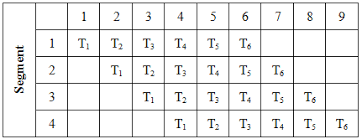
\includegraphics[scale=1]{images/pipeline.png} 
\caption{Design pattern \texttt{Pipeline}}
\end{center}
\end{figure}
Chaque tâche est donc complètement indépendante des autres. Ce design pattern est souvent associé à l'image du travail à la chaîne : un ouvrier effectue un traitement sur la pièce et la chaîne avance pour que le prochain traitement soit effectué. Ces tâches peuvent être exécutées de manière simultanée si le matériel le permet, à condition de respecter l'ordre des traitements et de ne pas effectuer deux tâches sur un même bloc dans le même intervalle de temps. En règle général en parallélisme, on affecte un processeur à une tâche afin de simplifier la modélisation.
\smallbreak
Cette modélisation semble être avantageuse mais pose des problèmes récurrents en parallélisme : comment définir l'ordre d'exécution des traitements sur un bloc ? Comment faire communiquer les étages du pipeline ?
\smallbreak
Afin de résoudre ces problèmes, on aura recours à la notion de parallélisme native en Ada avec les \texttt{task}.

\subsection{Notion de tâches en Ada}
Les tâches sont des éléments natifs de Ada et se caractérisent par une syntaxe particulière :
	\begin{lstlisting}[language=ada]
 task type IP_Task (Handler : Ptr_IPHandler) is
      entry Next_Task (Next_Step : Ptr_Feistel_Task);
      entry Process_Token (Token : T_BinaryBlock ; Id : Integer);
   end IP_Task;
	\end{lstlisting}
Une tâche est un type en Ada qui possède des \texttt{entry}. Les \texttt{entry} sont en fait des rendez-vous entre les tâches. Les rendez-vous sont utilisés pour la communication inter-tâche. A chaque fois qu'une tâche veut passer un bloc à une autre tâche, il faut qu'elle convienne d'un rendez-vous avec la tâche afin de passer ses données. Au delà des rendez-vous chaque tâche effectue son traitement de manière indépendante aux autres. Ainsi, des rendez-vous seront demandés à la fin de chaque traitement de tâche.
\smallbreak
Une tâche peut accepter un rendez-vous avec une autre tâche grâce à des \texttt{accept} qui permet d'accepter le rendez-vous avec une autre tâche. Ainsi avec cette dualité \texttt{accept}/\texttt{entry} on obtient une communication inter-tâches.

\subsection{Application du \texttt{Pipeline} à l'algorithme DES}
Pour l'algorithme DES, on a déjà évoqué le fait que l'entrée et la sortie n'étaient pas parallélisables car elles faisaient appel à une ressource critique (les fichier d'entrée/sortie). Cependant on a pu identifier les filtres comme pouvant être exécutés de manières indépendantes tant que l'ordre est respecté.
\smallbreak
Des modifications sont cependant nécessaires par rapport à la version séquentielle. Auparavant, les traitements étaient effectués sur tout le conteneur. Afin de paralléliser l'exécution, l'algorithme nécessite la fragmentation des données. Ainsi, pour chaque \texttt{Handler}, on définit une méthode \texttt{Process\_Block} qui effectue son traitement sur un seul bloc sans faire appel au prochain \texttt{Handler}. Finalement, on rend ce traitement plus élémentaire.
\smallbreak
Une fois les outils définis dans les \texttt{Handler}, on peut définir les tâches nécessaires à la construction du pipeline.

\subsection{Définition des tâches nécessaires au traitement}
Comme vu précédemment, on va définir une tâche par traitement grâce aux tâches Ada. Chaque tâche doit faire appel au prochain traitement à l'aide d'un rendez-vous et la dernière tâche doit placer le résultat dans le conteneur de donnée binaire.
\smallbreak
Pour arriver à ce résultat, on va définir les éléments qui circulent dans le pipeline. Afin de garder l'ordre des blocs, les éléments gérés par les tâches seront le couple bloc/index afin de pouvoir garder la position de ce bloc en mémoire et savoir où le placer en fin de traitement.
\smallbreak
Les tâches sont définies sur le même modèle : 
\begin{itemize}
\item Elles possèdent le \texttt{Handler} correspondant à leur traitement afin d'avoir accès au service nécessaire pour traiter le token
\item Elles possèdent un attribut pointeur vers la tâche suivante qui permet de connaître l'ordre d'exécution des filtres
\item Elles possèdent un attribut Token qui est le couple bloc/index qui sera traité
\item Elles peuvent accepter et envoyer des token dans le pipeline
\end{itemize}

Au final on aura 3 tâches :
\begin{itemize}
\item IP Task (transposition initiale)
\item Feistel Task (cycle de chiffrement)
\item Reverse IP (transposition finale)
\end{itemize}
Ci-dessous la définition complète de la tâche IP :
\newpage
	\begin{lstlisting}[language=ada]
   task body IP_Task is
      Next : Ptr_Feistel_Task;
      Block : T_BinaryBlock;
      Index : Integer;
   begin
      accept Next_Task (Next_Step : in Ptr_Feistel_Task) do
         Next := Next_Step;
      end Next_Task;
      
      loop
         select 
            accept Process_Token (Token : in T_BinaryBlock; Id : in Integer) do
               Block := Token;
               Index := Id;
            end Process_Token;
            Block := Handler.Process_Block (Block);
            Next.Process_Token (Block, Index);
            
            or
               terminate;
            end select;
      end loop;
	\end{lstlisting}
La tâche via son entrée \texttt{Next\_Task} va recevoir la tâche suivante et elle possède un \texttt{Handler} permettant d'effectuer le traitement. Ensuite, la boucle \texttt{select} et le statement \texttt{accept} va permettre de recevoir un bloc, de le traiter et de l'envoyer à la tâche suivante.

\subsection{Structure générale de l'algorithme}
La version séquentielle était assez simple en terme d'exécution. En appelant le premier \texttt{Handler}, on s'assure que la chaîne va être appelé jusqu'au bout. Dans la version parallèle il faut parcourir la conteneur de manière séquentielle mais on va envoyer des blocs dans le pipeline de tâche.
\smallskip
Le pipeline est considéré comme construit lorsque toutes les tâches ont reçu leur \texttt{Next\_Task}.

\begin{lstlisting}[language=ada]
   declare
      IP        : aliased IP_Task (IPLink'Unchecked_Access);
      Feistel   : aliased Feistel_Task (FeistelLink'Unchecked_Access);
      ReverseIP : aliased ReverseIP_Task (ReverseIPLink'Unchecked_Access);
      Output    : aliased Output_Task (OutputLink.Get_BinaryContainer);
   begin
      IP.Next_Task (Feistel'Unchecked_Access);
      Feistel.Next_Task (ReverseIP'Unchecked_Access);
      ReverseIP.Next_Task (Output'Unchecked_Access);
      
      for i in InputLink.Get_BinaryContainer'Range loop
         IP.Process_Token (InputLink.Get_BinaryContainer.all(i), i);
      end loop;
   end;
\end{lstlisting}
On peut ici voir une autre spécificité du langage Ada, les \texttt{Handler} étant définis dans un autre bloc de code, le compilateur restreint leur accès par pointeur. Cette mesure est prise afin de limiter le problème des dangling pointers. On doit donc avoir recours au \texttt{Unchecked\_Access} afin de forcer le compilateur à nous donner la référence de l'objet pointé.
\subsection{Limite de l'algorithme parallèle}
Les limites de l'algorithme parallèle sont multiples. Tout d'abords, certaines parties du code ne sont pas parallélisable (génération des clés qui sont nécessaires avant tout traitement, écriture et lecture des fichiers). De plus dans le cas de cet algorithme, les rendez-vous sont couteux en temps, de ce fait, le gain n'est pas très significatif. 
\smallbreak
De plus le comportement est beaucoup difficile à prévoir dans la version parallèle, les risques d'inter-blocages restent présents et le comportement peut changer en fonction du matériel et des directives du compilateur notamment.

\section{Conclusion}
En conclusion, l'algorithme implémenté de manière séquentielle comme parallèle est fonctionnelle. J'ai pu apprendre les difficultés du langage Ada ainsi que ses fonctionnalités mais également comprendre sa philosophie. Les pistes d'améliorations sont nombreuses, on pourrait mettre en place un profil Ravenscar qui permet de restreindre encore plus les opérations possibles et qui permet également d'effectuer une preuve formelle du programme.
\smallbreak
En conclusion ce projet m'a permis de me rendre compte des contraintes de programmation en temps réel ainsi que des limites et la portée de la mise en place d'un tel algorithme.



\end{document}
